% Created by tikzDevice version 0.12.6 on 2024-11-10 11:15:56
% !TEX encoding = UTF-8 Unicode
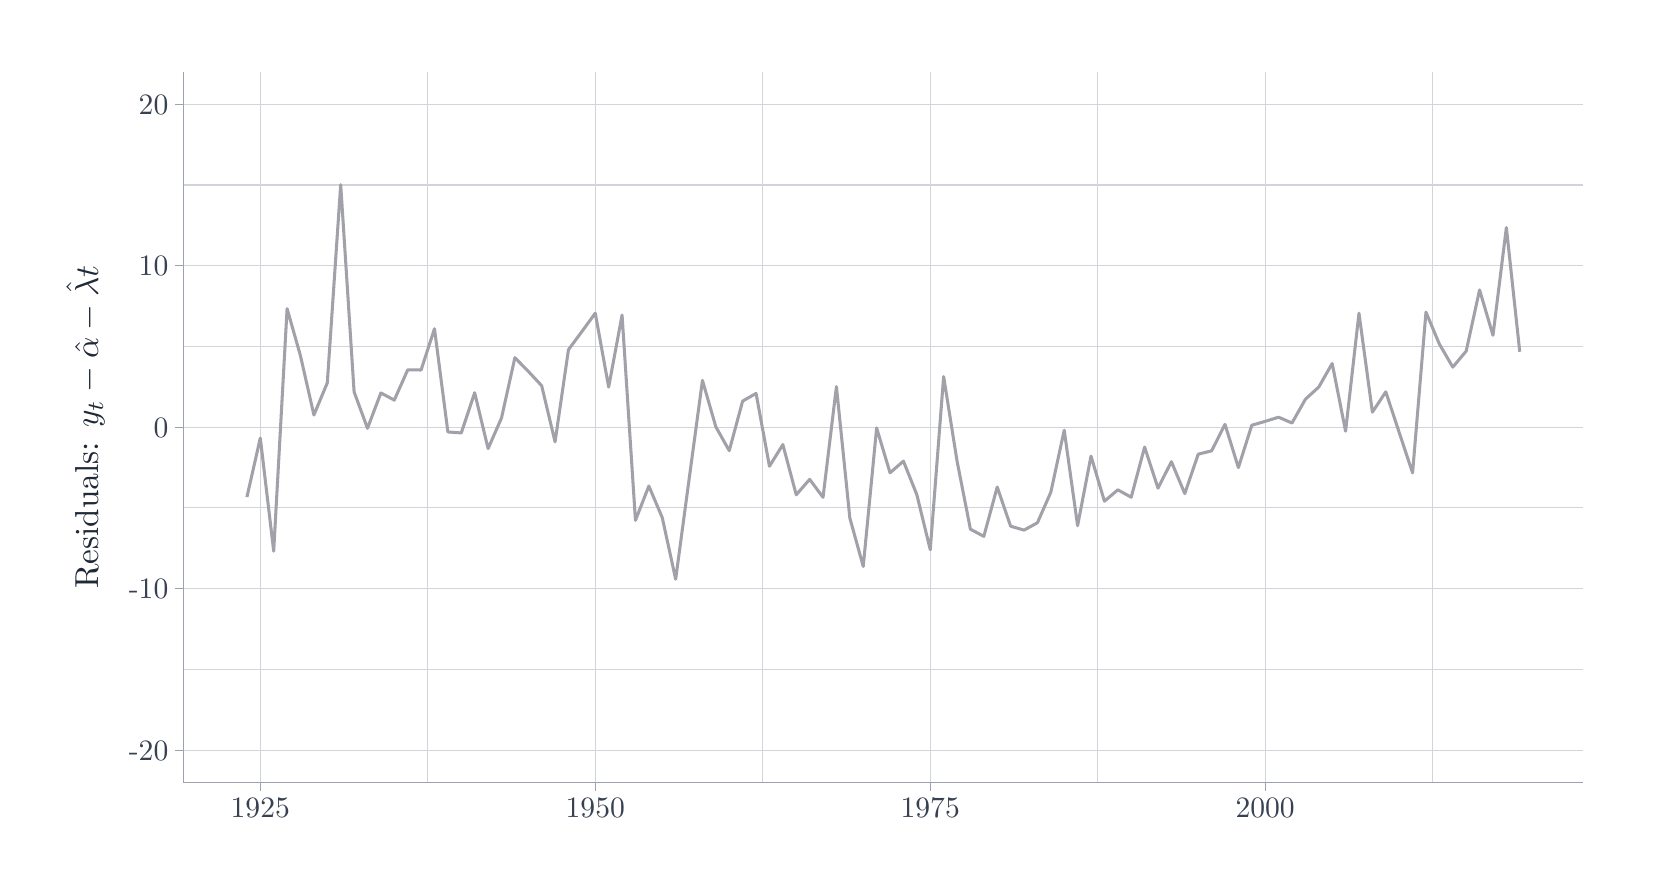
\begin{tikzpicture}[x=1pt,y=1pt]
\definecolor{fillColor}{RGB}{255,255,255}
\path[use as bounding box,fill=fillColor] (0,0) rectangle (578.16,303.53);
\begin{scope}
\path[clip] (  0.00,  0.00) rectangle (578.16,303.53);
\definecolor{drawColor}{RGB}{255,255,255}

\path[draw=drawColor,line width= 0.6pt,line join=round,line cap=round,fill=fillColor] ( -0.00,  0.00) rectangle (578.16,303.53);
\end{scope}
\begin{scope}
\path[clip] ( 56.22, 30.82) rectangle (562.16,287.53);
\definecolor{drawColor}{RGB}{255,255,255}
\definecolor{fillColor}{RGB}{255,255,255}

\path[draw=drawColor,line width= 0.6pt,line join=round,line cap=round,fill=fillColor] ( 56.22, 30.82) rectangle (562.16,287.53);
\definecolor{drawColor}{RGB}{209,213,219}

\path[draw=drawColor,line width= 0.4pt,line join=round] ( 56.22, 71.66) --
	(562.16, 71.66);

\path[draw=drawColor,line width= 0.4pt,line join=round] ( 56.22,130.01) --
	(562.16,130.01);

\path[draw=drawColor,line width= 0.4pt,line join=round] ( 56.22,188.35) --
	(562.16,188.35);

\path[draw=drawColor,line width= 0.4pt,line join=round] ( 56.22,246.69) --
	(562.16,246.69);

\path[draw=drawColor,line width= 0.4pt,line join=round] (144.58, 30.82) --
	(144.58,287.53);

\path[draw=drawColor,line width= 0.4pt,line join=round] (265.62, 30.82) --
	(265.62,287.53);

\path[draw=drawColor,line width= 0.4pt,line join=round] (386.65, 30.82) --
	(386.65,287.53);

\path[draw=drawColor,line width= 0.4pt,line join=round] (507.69, 30.82) --
	(507.69,287.53);

\path[draw=drawColor,line width= 0.4pt,line join=round] ( 56.22, 42.49) --
	(562.16, 42.49);

\path[draw=drawColor,line width= 0.4pt,line join=round] ( 56.22,100.83) --
	(562.16,100.83);

\path[draw=drawColor,line width= 0.4pt,line join=round] ( 56.22,159.18) --
	(562.16,159.18);

\path[draw=drawColor,line width= 0.4pt,line join=round] ( 56.22,217.52) --
	(562.16,217.52);

\path[draw=drawColor,line width= 0.4pt,line join=round] ( 56.22,275.87) --
	(562.16,275.87);

\path[draw=drawColor,line width= 0.4pt,line join=round] ( 84.06, 30.82) --
	( 84.06,287.53);

\path[draw=drawColor,line width= 0.4pt,line join=round] (205.10, 30.82) --
	(205.10,287.53);

\path[draw=drawColor,line width= 0.4pt,line join=round] (326.14, 30.82) --
	(326.14,287.53);

\path[draw=drawColor,line width= 0.4pt,line join=round] (447.17, 30.82) --
	(447.17,287.53);
\definecolor{drawColor}{RGB}{161,161,170}

\path[draw=drawColor,line width= 1.1pt,line join=round] ( 79.22,133.91) --
	( 84.06,155.24) --
	( 88.90,114.35) --
	( 93.74,202.00) --
	( 98.58,184.92) --
	(103.43,163.57) --
	(108.27,175.18) --
	(113.11,246.79) --
	(117.95,171.95) --
	(122.79,158.76) --
	(127.63,171.54) --
	(132.47,168.95) --
	(137.32,179.88) --
	(142.16,179.83) --
	(147.00,194.74) --
	(151.84,157.44) --
	(156.68,157.09) --
	(161.52,171.62) --
	(166.37,151.43) --
	(171.21,162.46) --
	(176.05,184.28) --
	(180.89,179.36) --
	(185.73,174.15) --
	(190.57,153.86) --
	(195.41,187.16) --
	(200.26,193.71) --
	(205.10,200.36) --
	(209.94,173.66) --
	(214.78,199.66) --
	(219.62,125.51) --
	(224.46,137.90) --
	(229.31,126.46) --
	(234.15,104.23) --
	(238.99,140.25) --
	(243.83,176.07) --
	(248.67,159.29) --
	(253.51,150.67) --
	(258.35,168.60) --
	(263.20,171.37) --
	(268.04,145.05) --
	(272.88,152.87) --
	(277.72,134.73) --
	(282.56,140.31) --
	(287.40,133.83) --
	(292.24,173.83) --
	(297.09,126.32) --
	(301.93,108.86) --
	(306.77,158.88) --
	(311.61,142.68) --
	(316.45,146.90) --
	(321.29,134.78) --
	(326.14,114.89) --
	(330.98,177.45) --
	(335.82,146.96) --
	(340.66,122.30) --
	(345.50,119.71) --
	(350.34,137.54) --
	(355.18,123.39) --
	(360.03,121.97) --
	(364.87,124.63) --
	(369.71,135.66) --
	(374.55,158.06) --
	(379.39,123.58) --
	(384.23,148.71) --
	(389.08,132.41) --
	(393.92,136.53) --
	(398.76,133.85) --
	(403.60,151.97) --
	(408.44,137.14) --
	(413.28,146.70) --
	(418.12,135.17) --
	(422.97,149.41) --
	(427.81,150.61) --
	(432.65,160.18) --
	(437.49,144.56) --
	(442.33,159.87) --
	(447.17,161.27) --
	(452.02,162.77) --
	(456.86,160.67) --
	(461.70,169.26) --
	(466.54,173.68) --
	(471.38,182.18) --
	(476.22,157.71) --
	(481.06,200.34) --
	(485.91,164.60) --
	(490.75,171.93) --
	(495.59,157.28) --
	(500.43,142.64) --
	(505.27,200.73) --
	(510.11,189.20) --
	(514.96,180.87) --
	(519.80,186.65) --
	(524.64,208.76) --
	(529.48,192.37) --
	(534.32,231.30) --
	(539.16,186.42);
\end{scope}
\begin{scope}
\path[clip] (  0.00,  0.00) rectangle (578.16,303.53);
\definecolor{drawColor}{RGB}{156,163,175}

\path[draw=drawColor,line width= 0.3pt,line join=round] ( 56.22, 30.82) --
	( 56.22,287.53);
\end{scope}
\begin{scope}
\path[clip] (  0.00,  0.00) rectangle (578.16,303.53);
\definecolor{drawColor}{RGB}{55,65,81}

\node[text=drawColor,anchor=base east,inner sep=0pt, outer sep=0pt, scale=  1.07] at ( 50.82, 38.82) {-20};

\node[text=drawColor,anchor=base east,inner sep=0pt, outer sep=0pt, scale=  1.07] at ( 50.82, 97.16) {-10};

\node[text=drawColor,anchor=base east,inner sep=0pt, outer sep=0pt, scale=  1.07] at ( 50.82,155.50) {0};

\node[text=drawColor,anchor=base east,inner sep=0pt, outer sep=0pt, scale=  1.07] at ( 50.82,213.85) {10};

\node[text=drawColor,anchor=base east,inner sep=0pt, outer sep=0pt, scale=  1.07] at ( 50.82,272.19) {20};
\end{scope}
\begin{scope}
\path[clip] (  0.00,  0.00) rectangle (578.16,303.53);
\definecolor{drawColor}{RGB}{156,163,175}

\path[draw=drawColor,line width= 0.3pt,line join=round] ( 53.22, 42.49) --
	( 56.22, 42.49);

\path[draw=drawColor,line width= 0.3pt,line join=round] ( 53.22,100.83) --
	( 56.22,100.83);

\path[draw=drawColor,line width= 0.3pt,line join=round] ( 53.22,159.18) --
	( 56.22,159.18);

\path[draw=drawColor,line width= 0.3pt,line join=round] ( 53.22,217.52) --
	( 56.22,217.52);

\path[draw=drawColor,line width= 0.3pt,line join=round] ( 53.22,275.87) --
	( 56.22,275.87);
\end{scope}
\begin{scope}
\path[clip] (  0.00,  0.00) rectangle (578.16,303.53);
\definecolor{drawColor}{RGB}{156,163,175}

\path[draw=drawColor,line width= 0.3pt,line join=round] ( 56.22, 30.82) --
	(562.16, 30.82);
\end{scope}
\begin{scope}
\path[clip] (  0.00,  0.00) rectangle (578.16,303.53);
\definecolor{drawColor}{RGB}{156,163,175}

\path[draw=drawColor,line width= 0.3pt,line join=round] ( 84.06, 27.82) --
	( 84.06, 30.82);

\path[draw=drawColor,line width= 0.3pt,line join=round] (205.10, 27.82) --
	(205.10, 30.82);

\path[draw=drawColor,line width= 0.3pt,line join=round] (326.14, 27.82) --
	(326.14, 30.82);

\path[draw=drawColor,line width= 0.3pt,line join=round] (447.17, 27.82) --
	(447.17, 30.82);
\end{scope}
\begin{scope}
\path[clip] (  0.00,  0.00) rectangle (578.16,303.53);
\definecolor{drawColor}{RGB}{55,65,81}

\node[text=drawColor,anchor=base,inner sep=0pt, outer sep=0pt, scale=  1.07] at ( 84.06, 18.07) {1925};

\node[text=drawColor,anchor=base,inner sep=0pt, outer sep=0pt, scale=  1.07] at (205.10, 18.07) {1950};

\node[text=drawColor,anchor=base,inner sep=0pt, outer sep=0pt, scale=  1.07] at (326.14, 18.07) {1975};

\node[text=drawColor,anchor=base,inner sep=0pt, outer sep=0pt, scale=  1.07] at (447.17, 18.07) {2000};
\end{scope}
\begin{scope}
\path[clip] (  0.00,  0.00) rectangle (578.16,303.53);
\definecolor{drawColor}{RGB}{31,41,55}

\node[text=drawColor,rotate= 90.00,anchor=base,inner sep=0pt, outer sep=0pt, scale=  1.20] at ( 25.43,159.18) {Residuals: $y_t - \hat{\alpha} - \hat{\lambda} t$};
\end{scope}
\end{tikzpicture}
